\subsection{Kleinste und grösste positive Zahlen}

Die Länge vom Seil (die Anzahl der möglichen Exponenten) und die Sitzplätze im Wagen (die verfügbaren Bits in der Mantisse) sind endlich. Deswegen können wir nur eine endliche Anzahl von Zahlen darstellen. Dann gibt es unter den endlich vielen positiven Zahlen eine grösste und eine kleinste.

\begin{beispiel}
Mantissenlänge: 5 Bits, Exponentenbereich: -3 bis 3.

Wie konstruieren wir die grösste Zahl?

Was wäre die Mantisse? So gross wie möglich. 1.1111

Was wäre der Exponent? So gross wie möglich. 3

Wagen-Darstellung:

Bitmuster: 0 111 (1)1111

Mathematische Darstellung: \(1.1111 \cdot 2^3\)

Wert: 15.5

\end{beispiel}

\begin{beispiel}
Mantissenlänge: 5 Bits, Exponentenbereich: -3 bis 3.

Wie konstruieren wir die kleinste Zahl?

Was wäre die Mantisse? So klein wie möglich, dennoch mit einer führenden Eins: 1.0000

Was wäre der Exponent? So klein wie möglich. -3

Wagen-Darstellung:

Bitmuster: 0 001 (1)0000

Mathematische Darstellung: \(1.0000 \cdot 2^{-3}\)

Wert: 1/8
\end{beispiel}

\begin{aufgabe}
Mantissenlänge: 3 Bits, Exponentenbereich: -1 bis 1.
Finde die grösste und kleinste positive Zahlen in diesem Fliesskommasystem. Stelle sie als Bitmuster und in der Exponentialschreibweise dar (Wert im Dezimalsystem angeben).
(Für den Exponentenbereich: 01 kodiert -1, 10 kodiert 0, 11 kodiert 1).
\end{aufgabe}

\begin{aufgabe}
Mantissenlänge: 4 Bits, Exponentenbereich: -1 bis 1, kodiert wie in der vorherigen Aufgabe.
Finde die grösste und kleinste positive Zahlen (Werte im Dezimalsystem angeben). Stelle sie als Bitmuster und in der Exponentialschreibweise dar.
\end{aufgabe}

Im Allgemeinen für einen Fliesskommasystem, wo die Mantisse m Bits lang ist und der Exponentenbereich von \(e_min\) bis \(e_max\) geht, findet man die grösste positive Zahl indem man in der Mantisse nur Einser schreibt, so dass diese so gross wie möglich wird: \(1.11111 \ldots 111\) und den Exponenten so gross wie möglich wählt: \(e_max\). Die grösste Zahl ist also:
\[1.1111111 \ldots 111 \cdot 2^{e_{max}}\]
Und hat den Bitmuster: 0 1111...11 (1)11111...11.

Die kleinste positive Zahl findet man, indem man die Mantisse so klein wie möglich wählt: \(1.00000 \ldots 000\) und den Exponenten so klein wie möglich: \(e_min\). Die kleinste Zahl ist also:
\[1.0000000 \ldots 000 \cdot 2^{e_{min}}\]
Und hat den Bitmuster: 0 0000...01 (1)000000...0.

\subsection{Darstellbare Zahlen}

In diesem Abschnitt werden wir ein Gefühl dafür bekommen, welche Zahlen sie darstellen lassen und welche nicht.
Hier und in den folgenden Kapiteln, falls nicht speziell vermerkt, werden wir mit Mantissenlänge 5 und Exponentenbereich von -3 bis 3 arbeiten.

\begin{beispiel}
Nehmen wir eine Zahl zwischen 1/8 und 15.5 (die kleinste und grösste darstellbare Zahlen in diesem Fliesskommasystem), zum Beispiel 10.25. Lässt sich diese Zahl darstellen?

[Bild mit Wagen]

Diese Zahl lässt sich in gegebenem System nicht exakt darstellen, weil in der Mantisse gibt es Platz nur für 5 Bits, so geht die letzte 1 verloren.
\end{beispiel}

\begin{beispiel}
Wir werden jetzt die nächste und die vorherige darstellbare Zahl von 1 finden.

[Bild mit Wagen]
\begin{figure}[H]
\centering
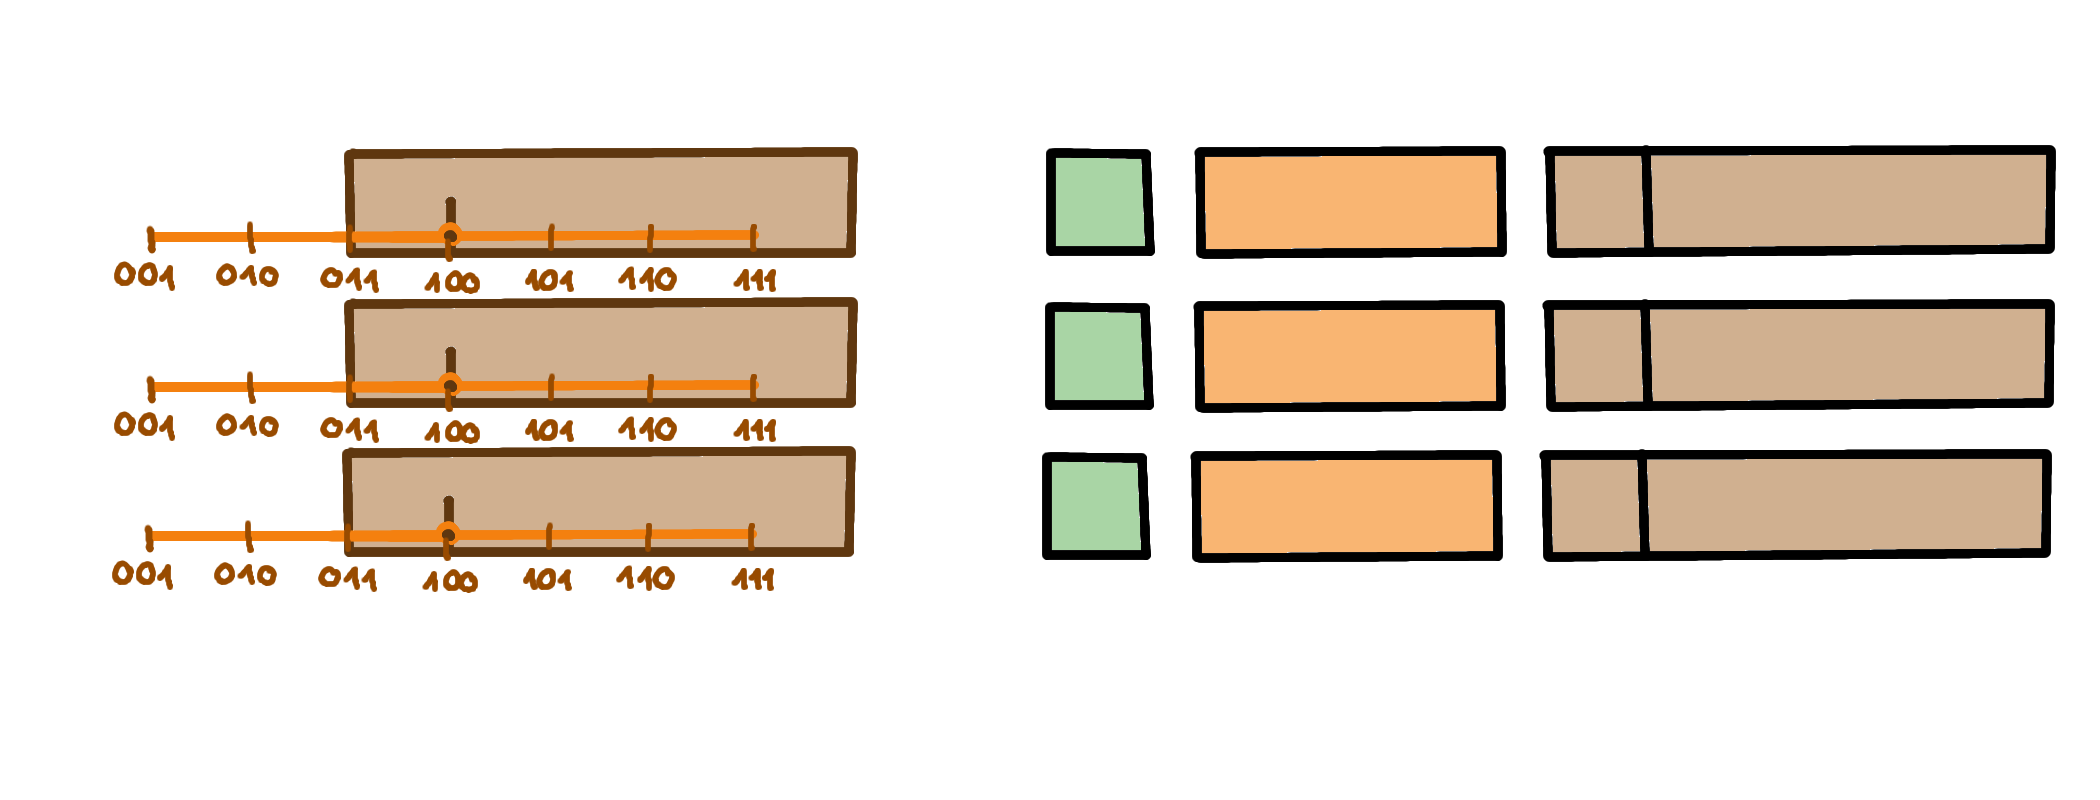
\includegraphics[width=\linewidth]{Pictures/Nachbarn.png} 
\end{figure}

Die nächste Zahl finden wir, indem wir in der Mantisse ganz rechts eine Eins setzen. Das ist die nächstgrösste Mantisse nach 1.0000. Der Exponent bleibt gleich. Die nächste Zahl ist also 1 + 1/16.

Die grösste Zahl kleiner als Eins finden wir, indem wir die Mantisse so gross wie möglich machen und den Exponenten um eins verkleinern. Die vorherige Zahl ist also 1 - 1/32.
\end{beispiel}

\begin{aufgabe}
Finde den nächstkleinsten und nächstgrössten darstellbaren Nachbar von den folgenden Zahlen. Schreibe die Werte im Dezimalsystem auf und stelle sie als Bitmuster und in der Exponentialschreibweise dar. Sind alle Nachbarn gleich entfernt?
\begin{enumerate}[(a)]
\item 2
\item 3
\item 4
\end{enumerate}
\end{aufgabe}

\subsubsection*{\textcolor{blue-violet}{Teste dich selber}}

\begin{aufgabe}\label{fliesskommazahlen_kontrollfragen}
Beantworte folgende Fragen:
\begin{enumerate}[(a)]
\item Kann man im Fliesskommazahlensystem alle reelle Zahlen darstellen?
\item Gibt es eine grösste Zahl im Fliesskommazahlensystem? Falls nein, warum? Falls ja, wie findet man sie?
\item Gibt es eine kleinste Zahl im Fliesskommazahlensystem? Falls nein, warum? Falls ja, wie findet man sie?
\item Warum kann man nicht alle Zahlen zwischen f\_min und f\_max darstellen? Gib ein Beispiel von einer Zahl, die sich nicht im System mit Mantissenlänge 3 und Exponentenbereich von -1 bis 1 darstellen lässt.
\item Sind alle Zahlen im Fliesskommazahlensystem gleichverteilt oder gibt es kleinere und grössere Löcher? Falls es Löcher gibt, wie sind sie verteilt? Wo sind sie grösser, wo sind sie kleiner?
\end{enumerate}
\end{aufgabe}
